\documentclass{article}

\usepackage[utf8]{inputenc}
\usepackage[spanish]{babel}
\usepackage[a4paper,top=2cm,bottom=2cm,left=3cm,right=3cm,marginparwidth=1.75cm]{geometry}
\usepackage{amsmath}
\usepackage{graphicx}
\graphicspath{{imagenes/}}
\usepackage{float}
\usepackage{caption}
\usepackage[colorlinks=true, allcolors=blue]{hyperref}

\title{\textbf{%
    Universidad Nacional de San Agustín \\
    Maestría en Ciencias de la Computación \\
    \large Análisis de Rendimiento de Algoritmos de Ordenamiento}}
\author{Abel Edmundo Borit Guitton, Luis Alberto Borit Guitton}
% \date{\today}
\date{1 de agosto de 2023}

\begin{document}
\maketitle

\section{INTRODUCCION}
\subsection{Introducción de algoritmos}
En informática, se llaman algoritmos el conjunto de instrucciones sistemáticas y previamente definidas que se utilizan para realizar una determinada tarea.

Se puede entender [1] un algoritmo como una secuencia de pasos finitos bien definidos que resuelven un problema. Por ejemplo, la ejecución de tareas cotidianas tan simples como cepillarse los dientes, lavarse las manos o seguir el manual de instrucciones de armado de un mueble, se pueden ver como un algoritmo.

\subsection{Introducción de Notación Big-O}
La [2] Notación Big-O es una forma de medir el tiempo lo bien que escala un programa o un algoritmo y el tiempo que tardará en ejecutar. Esta medición nos resultará muy útil para comparar la eficiencia de dos algoritmos, por ejemplo de ordenamiento.

\begin{figure}[h]
\centering
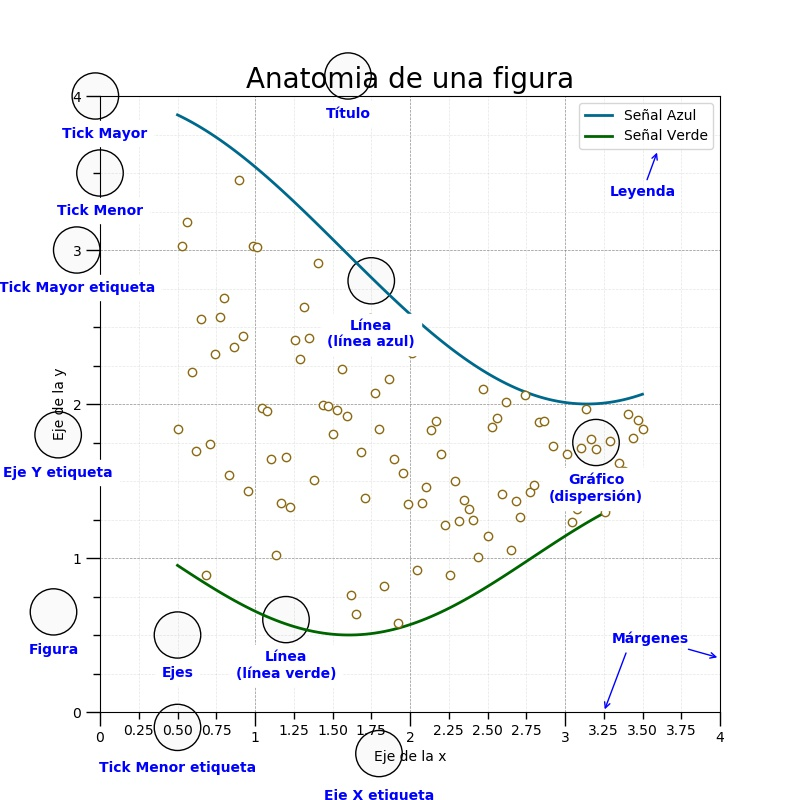
\includegraphics[width=0.6\textwidth]{Anatonia-de-un-grafico-matplotlibjpg.jpg}
\caption{\label{fig:matplotlib}Anatonia de un gráfico matplotlib}
\end{figure}

\subsection{Introducción de Matplotlib}
Matplotlib es una librería open source que pertenece a Python en la que se pueden crear visualizaciones animadas, estáticas e interactivas en Python. Se pueden usar gráficas con barras verticales, barras horizontales, líneas, etc.

\begin{figure}[h]
\centering
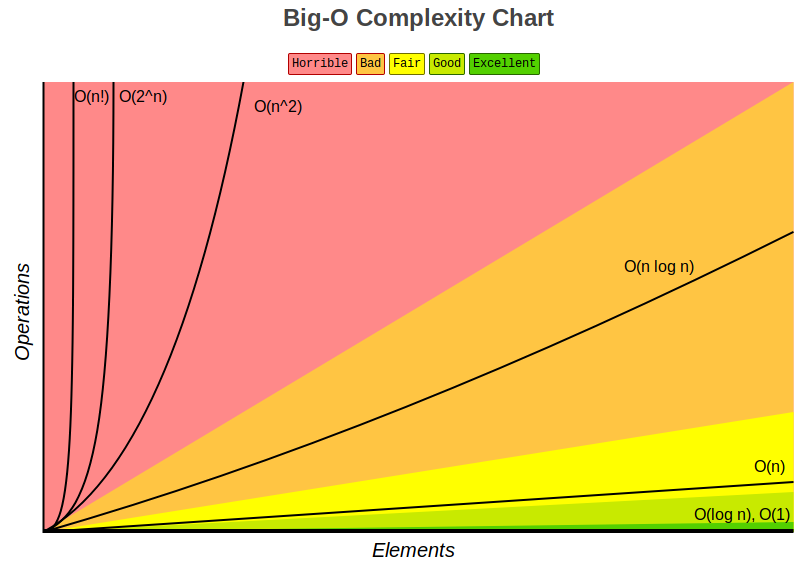
\includegraphics[width=0.6\textwidth]{big-o-complexity-chart.png}
\caption{\label{fig:bigo}Gráfico de complejidad BigO}
\end{figure}

% *****************************************************************

\section{ALGORITMOS}
\subsection{QUICK SORT}
[3] Quick sort es un algoritmo de ordenación basado en el enfoque divide y vencerás donde: Una matriz se divide en subarreglos seleccionando un elemento pivote (elemento seleccionado de la matriz). Al dividir la matriz, el elemento pivote debe colocarse de tal manera que los elementos menores que el pivote se mantengan en el lado izquierdo y los elementos mayores que el pivote estén en el lado derecho del pivote. Los subarreglos izquierdo y derecho también se dividen utilizando el mismo enfoque. Este proceso continúa hasta que cada subarreglo contiene un solo elemento. En este punto, los elementos ya están ordenados. Finalmente, los elementos se combinan para formar una matriz ordenada.

    \begin{table}[h!]
        \centering
        \begin{tabular}{||c c c c c||} 
         \hline
         \textbf{Algoritmo} & \textbf{Mejor caso} & \textbf{Peor caso} & \textbf{Promedio} & \textbf{Método} \\ [0.5ex] 
         \hline\hline
         Quick Sort & O(n*log n) & \(O(n^2)\) & O(n*log n) & Partición \\ [0.5ex] 
         \hline
        \end{tabular}
        \caption{Costo computacional Quick Sort.}
        \label{table:dataQuickSort}
    \end{table}

    \begin{enumerate}
        \item \textbf{Complejidad en el peor de los casos \(O(n^2)\):} Ocurre cuando el elemento pivote seleccionado es el elemento más grande o el más pequeño. Esta condición conduce al caso en el que el elemento pivote se encuentra en un extremo de la matriz ordenada. Un subconjunto siempre está vacío y otro subconjunto contiene n - 1 elementos. Por lo tanto, quicksort se llama solo en este subarreglo. Sin embargo, el algoritmo de clasificación rápida tiene un mejor rendimiento para pivotes dispersos.
        
        \item \textbf{Complejidad en el mejor de los casos O(n*log n):} Ocurre cuando el elemento pivote es siempre el elemento central o está cerca del elemento central.
        
        \item \textbf{Complejidad de caso promedio O(n*log n):} Ocurre cuando las condiciones anteriores no ocurren.
    \end{enumerate}
        
\subsection{MERGE SORT}
[4] Merge Sort es uno de los algoritmos de ordenación más populares que se basa en el principio del algoritmo divide y vencerás. El método de ordenamiento MergeSort funciona dividiendo una matriz en subarreglos más pequeños, ordenando cada subarreglo y luego fusionando los subarreglos ordenados para formar el arreglo ordenado final. En términos simples, podemos decir que el proceso de ordenación por fusión consiste en dividir la matriz en dos mitades, ordenar cada mitad y luego volver a unir las mitades ordenadas. Este proceso se repite hasta que se ordena toda la matriz.

    \begin{table}[H]
        \centering
        \begin{tabular}{||c c c c c||} 
         \hline
         \textbf{Algoritmo} & \textbf{Mejor caso} & \textbf{Peor caso} & \textbf{Promedio} & \textbf{Método} \\ [0.5ex] 
         \hline\hline
         Merge Sort & O(n*log n) & O(n*log n) & O(n*log n) & Mezcla \\ [0.5ex] 
         \hline
        \end{tabular}
        \caption{Costo computacional Merge Sort.}
        \label{table:dataMergeSort}
    \end{table}
    
    \begin{enumerate}
            \item \textbf{Complejidad del mejor caso O(n*log n):} Si la matriz ya está ordenada, entonces no hay necesidad de ordenar.
            
            \item \textbf{Complejidad en el peor de los casos O(n*log n):} Cuando el arreglo está completamente desordenado. En este caso, Merge Sort debe realizar todas las divisiones y combinaciones (merge) necesarias para ordenar el arreglo.
            
            \item \textbf{Complejidad promedio del caso O(n*log n):} Merge Sort tiene una característica constante en su complejidad, lo que significa que independientemente de los datos de entrada, la fase de división siempre dividirá el arreglo a la mitad y la fase de combinación (merge) combinará las sublistas en el orden correcto.
    \end{enumerate}

\subsection{BUBBLE SORT}
[5] Bubble sort es un algoritmo de ordenación que compara dos elementos adyacentes y los intercambia hasta que están en el orden previsto. Funciona revisando cada elemento de la lista que va a ser ordenada con el siguiente, intercambiándolos de posición si están en el orden equivocado. Es necesario revisar varias veces toda la lista hasta que no se necesiten más intercambios, lo cual significa que la lista está ordenada. Este algoritmo obtiene su nombre de la forma con la que suben por la lista los elementos durante los intercambios, como si fueran pequeñas "burbujas".

    \begin{table}[H]
        \centering
        \begin{tabular}{||c c c c c||} 
         \hline
         \textbf{Algoritmo} & \textbf{Mejor caso} & \textbf{Peor caso} & \textbf{Promedio} & \textbf{Método} \\ [0.5ex] 
         \hline\hline
         Bubble Sort & O(n) & \(O(n^2)\) & \(O(n^2)\) & Intercambio \\ [0.5ex] 
         \hline
        \end{tabular}
        \caption{Costo computacional Bubble Sort.}
        \label{table:dataBubbleSort}
    \end{table}
    
    \begin{enumerate}
            \item \textbf{Complejidad en el mejor de los casos: O(n):} Si la matriz ya está ordenada, entonces no hay necesidad de ordenar.
            
            \item \textbf{Complejidad del peor de los casos \(O(n^2)\):} Si queremos ordenar en orden ascendente y la matriz está en orden descendente, ocurre el peor de los casos.
            
            \item \textbf{Complejidad de caso promedio \(O(n^2)\):} Ocurre cuando los elementos de la matriz están en orden desordenado (ni ascendente ni descendente).
    \end{enumerate}

\subsection{SELECTION SORT}
[6] Selection sort es un algoritmo de ordenación que selecciona el elemento más pequeño de una lista sin ordenar en cada iteración y coloca ese elemento al principio de la lista sin ordenar. Es decir, busca el mínimo elemento de la lista, lo intercambia con el primero, luego busca el siguiente mínimo en el resto de la lista, después intercambiarlo con el segundo.

    \begin{table}[H]
        \centering
        \begin{tabular}{||c c c c c||} 
         \hline
         \textbf{Algoritmo} & \textbf{Mejor caso} & \textbf{Peor caso} & \textbf{Promedio} & \textbf{Método} \\ [0.5ex] 
         \hline\hline
         Selection Sort & \(O(n^2)\) & \(O(n^2)\) & \(O(n^2)\) & Intercambio \\ [0.5ex] 
         \hline
        \end{tabular}
        \caption{Costo computacional Selection Sort.}
        \label{table:dataSelectionSort}
    \end{table}
    
    \begin{enumerate}
            \item \textbf{Complejidad del peor de los casos \(O(n^2)\):} Si queremos ordenar en orden ascendente y la matriz está en orden descendente, entonces ocurre el peor de los casos.
            
            \item \textbf{Complejidad en el mejor de los casos \(O(n^2)\):} Ocurre cuando la matriz ya está ordenada.
            
            \item \textbf{Complejidad de caso promedio \(O(n^2)\):} Ocurre cuando los elementos de la matriz están en orden desordenado (ni ascendente ni descendente).
    \end{enumerate}

    
\subsection{COMPARACIÓN DE COSTO COMPUTACIONAL DE ALGORITMOS}

    \begin{table}[H]
        \centering
        \begin{tabular}{||c c c c c||} 
         \hline
         \textbf{Algoritmo} & \textbf{Mejor caso} & \textbf{Peor caso} & \textbf{Promedio} & \textbf{Método} \\ [0.5ex] 
         \hline\hline
          Quick Sort & O(n*log n) & \(O(n^2)\) & O(n*log n) & Partición \\ [0.5ex]
          Merge Sort & O(n*log n) & O(n*log n) & O(n*log n) & Mezcla \\ [0.5ex] 
          Bubble Sort & O(n) & \(O(n^2)\) & \(O(n^2)\) & Intercambio \\ [0.5ex]  
          Selection Sort & \(O(n^2)\) & \(O(n^2)\) & \(O(n^2)\) & Intercambio \\ [0.5ex]  
         \hline
        \end{tabular}
        \caption{Costo computacional comparación.}
        \label{table:dataComparationSorts}
    \end{table}

% *****************************************************************

\section{IMPLEMENTACION}
En el siguiente enlace \href{https://github.com/abelborit/computer-science-master/tree/main/MCC-01_algorithms-and-data-structures}{Repositorio GitHub} se podrá visualizar toda la implementación realizada. Cuenta con un file system estructurado para cada algoritmo usado, archivos txt de donde se tomarán los datos de entrada para los algoritmos, una carpeta donde está el código usado para realizar gráficas con el Matplotlib como sus gráficas correspondientes y también un archivo README.md propio del proyecto y repositorio.

\section{RESULTADOS}
\subsection{QUICK SORT}
    \begin{itemize}
      \item \textbf{TIEMPO PROMEDIO DE EJECUCIÓN (milisegundos):}
        \begin{table}[H]
            \centering
            \begin{tabular}{||c c c c||} 
              \hline
              \textbf{Cantidad de entrada de datos} & \textbf{PYTHON} & \textbf{GOLANG (GO)} & \textbf{C++} \\ [0.5ex] 
              \hline\hline
              100    &  0.04685001  &  0.000000  &  0.079910  \\ [0.5ex]
              1000   &  0.67782998  &  0.464720  &  1.148020  \\ [0.5ex]
              2000   &  1.43169999  &  0.602610  &  1.854120  \\ [0.5ex]
              3000   &  3.91183998  &  1.073230  &  3.110650  \\ [0.5ex]
              4000   &  4.84377998  &  1.265420  &  3.530010  \\ [0.5ex]
              5000   &  6.46152000  &  1.694050  &  4.680750  \\ [0.5ex]
              6000   &  7.95723999  &  4.598390  &  5.289930  \\ [0.5ex]
              7000   &  8.97102001  &  2.551000  &  5.995160  \\ [0.5ex]
              8000   &  10.2722399  &  2.075420  &  7.492810  \\ [0.5ex]
              9000   &  8.47290002  &  2.830250  &  8.306410  \\ [0.5ex]
              10000  &  11.0587500  &  2.955840  &  13.69270  \\ [0.5ex]
              20000  &  28.8310900  &  5.702930  &  17.39720  \\ [0.5ex]
              30000  &  36.8985099  &  8.255000  &  27.60360  \\ [0.5ex]
              40000  &  43.5867699  &  11.61944  &  40.43740  \\ [0.5ex]
              50000  &  54.3271499  &  13.76548  &  50.62150  \\ [0.5ex]
              \hline
            \end{tabular}
            \caption{Tiempo Promedio de ejecución (milisegundos) QUICK SORT.}
            \label{table:tiempoPromedioQuickSort}
        \end{table}

      \item \textbf{DESVIACIÓN ESTANDAR (milisegundos):}
        \begin{table}[H]
            \centering
            \begin{tabular}{||c c c c||} 
              \hline
              \textbf{Cantidad de entrada de datos} & \textbf{PYTHON} & \textbf{GOLANG (GO)} & \textbf{C++} \\ [0.5ex] 
              \hline\hline
              100    &  0.01237272  &  0.000000  &  0.007999  \\ [0.5ex]
              1000   &  0.04316520  &  0.185783  &  0.358207  \\ [0.5ex]
              2000   &  0.16441244  &  0.241817  &  0.296759  \\ [0.5ex]
              3000   &  0.33035275  &  0.294967  &  0.571884  \\ [0.5ex]
              4000   &  0.23674186  &  0.612106  &  0.289619  \\ [0.5ex]
              5000   &  0.29286814  &  0.490390  &  0.617485  \\ [0.5ex]
              6000   &  0.47211768  &  6.061293  &  0.459793  \\ [0.5ex]
              7000   &  0.29674173  &  0.724635  &  0.349818  \\ [0.5ex]
              8000   &  0.30146304  &  0.691155  &  0.620507  \\ [0.5ex]
              9000   &  2.58117163  &  0.608914  &  0.528023  \\ [0.5ex]
              10000  &  3.15333205  &  0.782962  &  4.817980  \\ [0.5ex]
              20000  &  0.89344093  &  0.907001  &  0.672907  \\ [0.5ex]
              30000  &  9.15402969  &  1.961678  &  0.808213  \\ [0.5ex]
              40000  &  10.5534478  &  4.393168  &  6.989210  \\ [0.5ex]
              50000  &  10.5772942  &  3.511714  &  7.839530  \\ [0.5ex]
              \hline
            \end{tabular}
            \caption{Desviación Estandar (milisegundos) QUICK SORT.}
            \label{table:desviacionEstandarQuickSort}
        \end{table}
    \end{itemize}

    \begin{figure}[H]
    \centering
    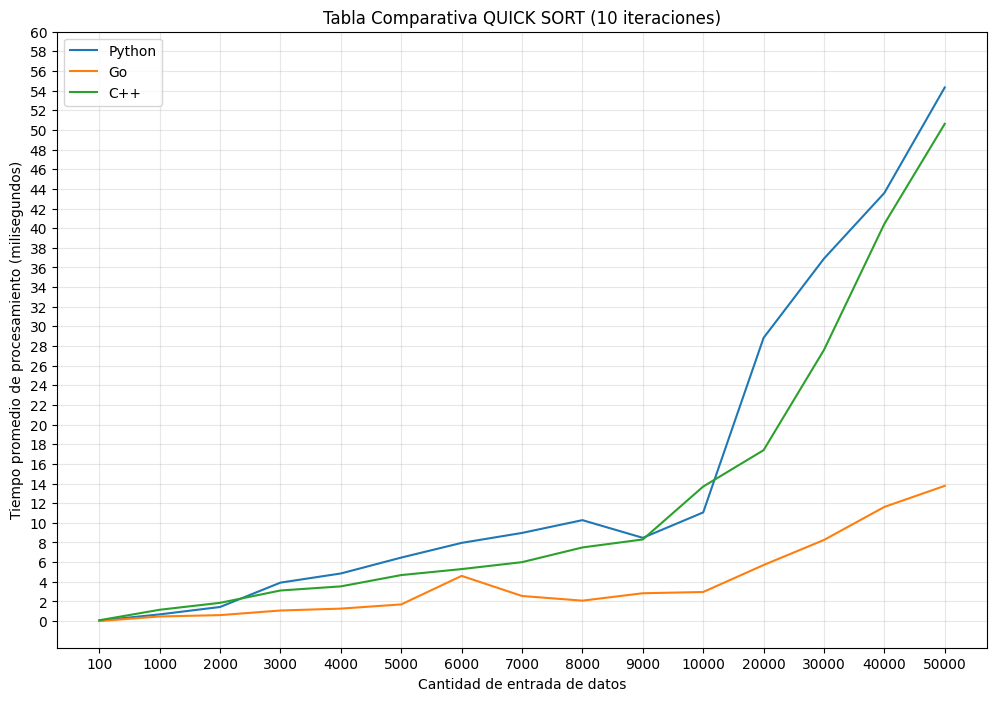
\includegraphics[width=0.95\textwidth]{GraphicQuickSort.png}
    \caption{\label{fig:bigOQuickSort}Gráfica comparativa Big-O del tiempo promedio de Ejecución Quick Sort}
    \end{figure}

\subsection{MERGE SORT}
    \begin{itemize}
      \item \textbf{TIEMPO PROMEDIO DE EJECUCIÓN (milisegundos):}
        \begin{table}[H]
            \centering
            \begin{tabular}{||c c c c||} 
              \hline
              \textbf{Cantidad de entrada de datos} & \textbf{PYTHON} & \textbf{GOLANG (GO)} & \textbf{C++} \\ [0.5ex] 
              \hline\hline
              100    &  0.099130010  &  0.000000  &  0.078730  \\ [0.5ex]
              1000   &  2.200649976  &  0.169101  &  0.962090  \\ [0.5ex]
              2000   &  2.764629971  &  0.604000  &  1.644030  \\ [0.5ex]
              3000   &  7.101050007  &  0.768830  &  2.564250  \\ [0.5ex]
              4000   &  9.642669999  &  0.984660  &  3.543940  \\ [0.5ex]
              5000   &  10.99956997  &  1.172470  &  5.469300  \\ [0.5ex]
              6000   &  14.79182001  &  1.439510  &  7.223770  \\ [0.5ex]
              7000   &  15.05678002  &  1.487160  &  6.174310  \\ [0.5ex]
              8000   &  16.64215999  &  1.975560  &  8.942220  \\ [0.5ex]
              9000   &  18.01923997  &  2.319490  &  10.56892  \\ [0.5ex]
              10000  &  22.10480999  &  2.148190  &  12.54333  \\ [0.5ex]
              20000  &  38.02304002  &  3.887100  &  21.78842  \\ [0.5ex]
              30000  &  62.77080999  &  5.903180  &  28.89253  \\ [0.5ex]
              40000  &  90.29701001  &  7.860120  &  37.25581  \\ [0.5ex]
              50000  &  115.8760799  &  10.38625  &  48.43261  \\ [0.5ex]
              \hline
            \end{tabular}
            \caption{Tiempo Promedio de ejecución (milisegundos) MERGE SORT.}
            \label{table:tiempoPromedioMergeSort}
        \end{table}

      \item \textbf{DESVIACIÓN ESTANDAR (milisegundos):}
        \begin{table}[H]
            \centering
            \begin{tabular}{||c c c c||} 
              \hline
              \textbf{Cantidad de entrada de datos} & \textbf{PYTHON} & \textbf{GOLANG (GO)} & \textbf{C++} \\ [0.5ex] 
              \hline\hline
              100    &  0.010380018  &  0.000000  &  0.012475  \\ [0.5ex]
              1000   &  0.139699127  &  0.274719  &  0.256427  \\ [0.5ex]
              2000   &  0.143155381  &  0.479039  &  0.173328  \\ [0.5ex]
              3000   &  0.252419432  &  0.557514  &  0.104371  \\ [0.5ex]
              4000   &  0.462389638  &  0.582344  &  0.509137  \\ [0.5ex]
              5000   &  2.069747269  &  0.370153  &  1.325930  \\ [0.5ex]
              6000   &  0.678121567  &  0.642554  &  1.784810  \\ [0.5ex]
              7000   &  2.711879093  &  0.574327  &  0.829839  \\ [0.5ex]
              8000   &  3.366178232  &  0.631392  &  2.279170  \\ [0.5ex]
              9000   &  4.311885757  &  0.727693  &  3.676050  \\ [0.5ex]
              10000  &  0.479471792  &  0.975979  &  5.137400  \\ [0.5ex]
              20000  &  7.918874973  &  0.794502  &  9.211090  \\ [0.5ex]
              30000  &  15.37298311  &  2.743981  &  10.15870  \\ [0.5ex]
              40000  &  20.97384071  &  3.730722  &  4.930550  \\ [0.5ex]
              50000  &  22.32296576  &  0.939189  &  9.778050  \\ [0.5ex]
              \hline
            \end{tabular}
            \caption{Desviación Estandar (milisegundos) MERGE SORT.}
            \label{table:desviacionEstandarMergeSort}
        \end{table}
    \end{itemize}

    \begin{figure}[H]
    \centering
    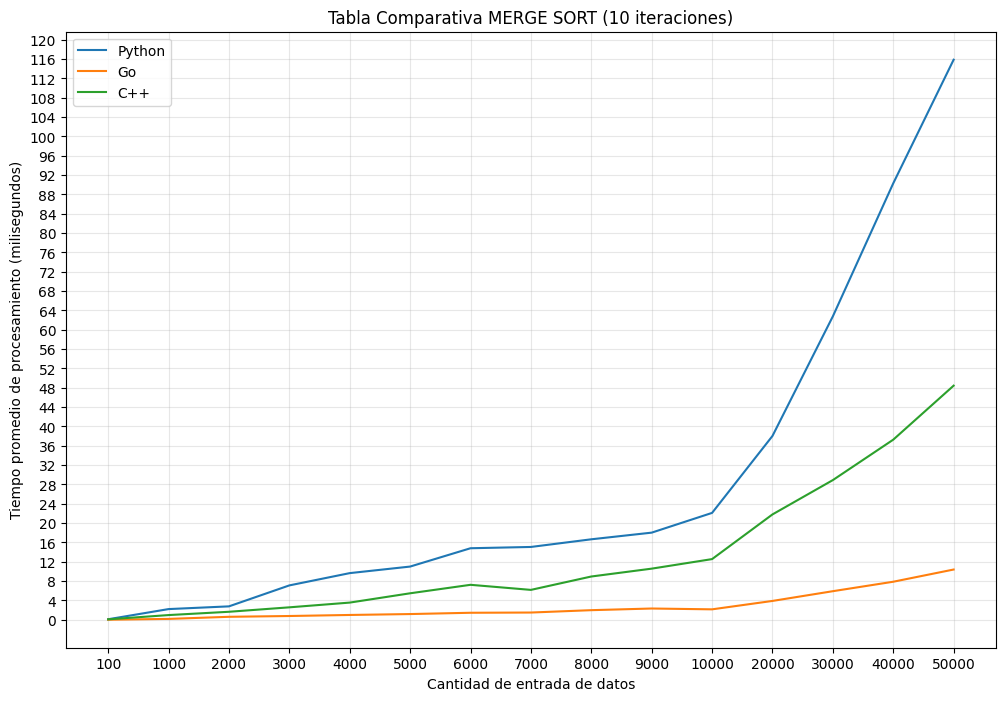
\includegraphics[width=0.95\textwidth]{GraphicMergeSort.png}
    \caption{\label{fig:bigOMergeSort}Gráfica comparativa Big-O del tiempo promedio de Ejecución Merge Sort}
    \end{figure}

\subsection{BUBBLE SORT}
    \begin{itemize}
      \item \textbf{TIEMPO PROMEDIO DE EJECUCIÓN (milisegundos):}
        \begin{table}[H]
            \centering
            \begin{tabular}{||c c c c||} 
              \hline
              \textbf{Cantidad de entrada de datos} & \textbf{PYTHON} & \textbf{GOLANG (GO)} & \textbf{C++} \\ [0.5ex] 
              \hline\hline
              100    &  0.09968999624  &  0.000000000  &  0.0049100  \\ [0.5ex]
              1000   &  6.85737999677  &  0.826706101  &  0.5218900  \\ [0.5ex]
              2000   &  33.6971200227  &  2.727610201  &  1.8218900  \\ [0.5ex]
              3000   &  48.8158600091  &  6.158550102  &  3.9607600  \\ [0.5ex]
              4000   &  102.356639993  &  11.68364003  &  11.797200  \\ [0.5ex]
              5000   &  205.870879995  &  17.17712001  &  16.963400  \\ [0.5ex]
              6000   &  224.816080021  &  25.98638001  &  22.042600  \\ [0.5ex]
              7000   &  407.337369978  &  32.83727002  &  27.552800  \\ [0.5ex]
              8000   &  463.472159981  &  43.07511001  &  34.134210  \\ [0.5ex]
              9000   &  639.334340012  &  54.13579002  &  41.019610  \\ [0.5ex]
              10000  &  768.145850014  &  63.22702005  &  53.374720  \\ [0.5ex]
              20000  &  3133.96456001  &  374.1022104  &  206.83610  \\ [0.5ex]
              30000  &  6707.64185004  &  954.4675301  &  459.03430  \\ [0.5ex]
              40000  &  12568.0394800  &  1800.399530  &  808.95120  \\ [0.5ex]
              50000  &  20324.6212799  &  2886.457870  &  1254.6610  \\ [0.5ex]
              \hline
            \end{tabular}
            \caption{Tiempo Promedio de ejecución (milisegundos) BUBBLE SORT.}
            \label{table:tiempoPromedioBubbleSort}
        \end{table}

      \item \textbf{DESVIACIÓN ESTANDAR (milisegundos):}
        \begin{table}[H]
            \centering
            \begin{tabular}{||c c c c||} 
              \hline
              \textbf{Cantidad de entrada de datos} & \textbf{PYTHON} & \textbf{GOLANG (GO)} & \textbf{C++} \\ [0.5ex] 
              \hline\hline
              100    &  0.2728753034297  &  0.0000000  &  0.01283351  \\ [0.5ex]
              1000   &  21.476972639436  &  0.2602590  &  1.54954102  \\ [0.5ex]
              2000   &  106.17322396426  &  0.4750190  &  5.44924101  \\ [0.5ex]
              3000   &  153.69314189604  &  0.4310630  &  11.8489201  \\ [0.5ex]
              4000   &  322.79907632474  &  0.7802910  &  35.3547101  \\ [0.5ex]
              5000   &  649.87024634287  &  0.7152800  &  50.8431303  \\ [0.5ex]
              6000   &  709.60714569460  &  4.2671250  &  66.0707104  \\ [0.5ex]
              7000   &  1286.6749632257  &  1.9363900  &  82.5959203  \\ [0.5ex]
              8000   &  1464.0974316437  &  2.2937910  &  102.338102  \\ [0.5ex]
              9000   &  2019.9168933881  &  2.3371280  &  122.984101  \\ [0.5ex]
              10000  &  2427.1399332939  &  3.2064260  &  160.044202  \\ [0.5ex]
              20000  &  9906.4383931220  &  7.7742460  &  620.347201  \\ [0.5ex]
              30000  &  21205.626498015  &  9.2817060  &  1376.87111  \\ [0.5ex]
              40000  &  39735.964451084  &  31.545510  &  2426.54121  \\ [0.5ex]
              50000  &  64264.998022662  &  14.926888  &  3763.59214  \\ [0.5ex]
              \hline
            \end{tabular}
            \caption{Desviación Estandar (milisegundos) BUBBLE SORT.}
            \label{table:desviacionEstandarBubbleSort}
        \end{table}
    \end{itemize}

    \begin{figure}[H]
    \centering
    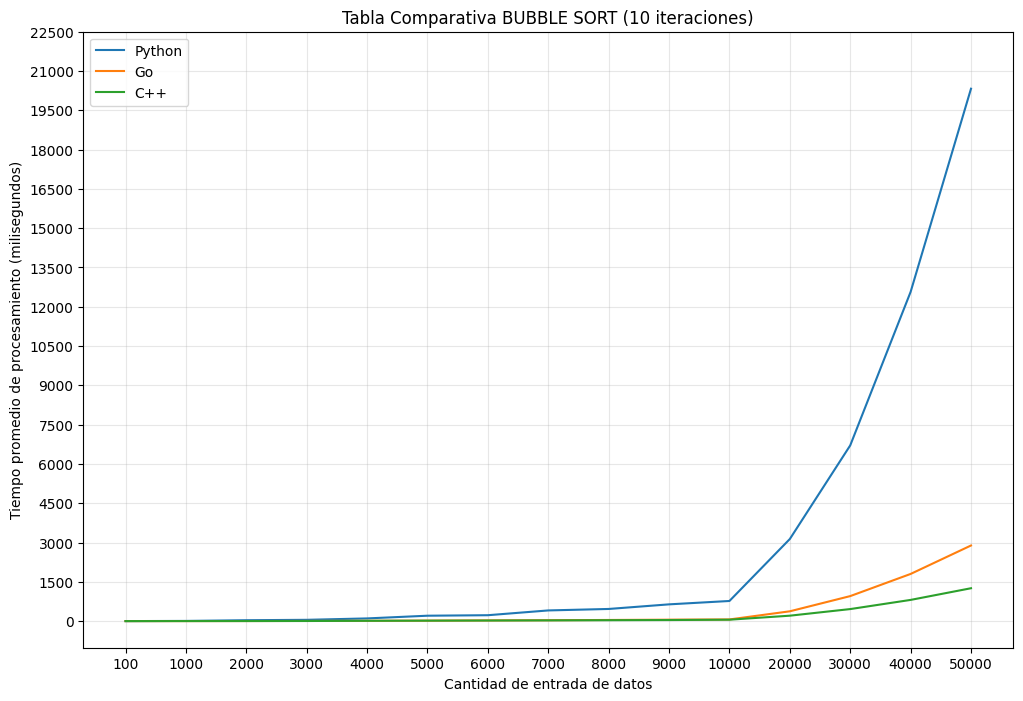
\includegraphics[width=0.95\textwidth]{GraphicBubbleSort.png}
    \caption{\label{fig:bigOBubbleSort}Gráfica comparativa Big-O del tiempo promedio de Ejecución Bubble Sort}
    \end{figure}

\subsection{SELECTION SORT}
    \begin{itemize}
      \item \textbf{TIEMPO PROMEDIO DE EJECUCIÓN (milisegundos):}
        \begin{table}[H]
            \centering
            \begin{tabular}{||c c c c||} 
              \hline
              \textbf{Cantidad de entrada de datos} & \textbf{PYTHON} & \textbf{GOLANG (GO)} & \textbf{C++} \\ [0.5ex] 
              \hline\hline
              100    &  0.126609981060  &  0.000000000  &  0.016970   \\ [0.5ex]
              1000   &  21.82428001165  &  0.494940010  &  1.655700   \\ [0.5ex]
              2000   &  62.14085003137  &  1.958650010  &  5.411630   \\ [0.5ex]
              3000   &  183.2173200368  &  4.028720020  &  11.81160   \\ [0.5ex]
              4000   &  311.7560799837  &  6.813090020  &  21.21250   \\ [0.5ex]
              5000   &  486.3501099705  &  10.64910010  &  32.61910   \\ [0.5ex]
              6000   &  681.5701000094  &  16.86822030  &  44.96860   \\ [0.5ex]
              7000   &  958.1987799644  &  21.20322001  &  63.97320   \\ [0.5ex]
              8000   &  1193.260069942  &  27.08228100  &  80.754915  \\ [0.5ex]
              9000   &  1646.823350012  &  33.87629010  &  104.23141  \\ [0.5ex]
              10000  &  1928.187919998  &  42.38623002  &  127.11545  \\ [0.5ex]
              20000  &  7124.636140012  &  167.3506101  &  499.09814  \\ [0.5ex]
              30000  &  16785.25921000  &  373.4584401  &  1116.4115  \\ [0.5ex]
              40000  &  32140.98073002  &  672.7258502  &  1978.6634  \\ [0.5ex]
              50000  &  47437.90182001  &  1035.016770  &  3118.5751  \\ [0.5ex]
              \hline
            \end{tabular}
            \caption{Tiempo Promedio de ejecución (milisegundos) SELECTION SORT.}
            \label{table:tiempoPromedioSelectionSort}
        \end{table}

      \item \textbf{DESVIACIÓN ESTANDAR (milisegundos):}
        \begin{table}[H]
            \centering
            \begin{tabular}{||c c c c||} 
              \hline
              \textbf{Cantidad de entrada de datos} & \textbf{PYTHON} & \textbf{GOLANG (GO)} & \textbf{C++} \\ [0.5ex] 
              \hline\hline
              100    &  0.005510114127  &  0.000000  &  0.0036883  \\ [0.5ex]
              1000   &  3.295351090810  &  0.184424  &  0.2727011  \\ [0.5ex]
              2000   &  18.07971368402  &  0.568659  &  0.6753572  \\ [0.5ex]
              3000   &  34.33263888649  &  0.500249  &  0.9801920  \\ [0.5ex]
              4000   &  92.37778663832  &  2.230710  &  3.0358901  \\ [0.5ex]
              5000   &  138.0157493079  &  0.966028  &  1.1607201  \\ [0.5ex]
              6000   &  143.9102225896  &  1.900818  &  0.9227041  \\ [0.5ex]
              7000   &  124.2825314188  &  1.500438  &  3.8177510  \\ [0.5ex]
              8000   &  186.9522389275  &  5.183933  &  1.8764920  \\ [0.5ex]
              9000   &  173.5418382981  &  4.867653  &  1.6594622  \\ [0.5ex]
              10000  &  284.1773666568  &  2.534389  &  3.7231501  \\ [0.5ex]
              20000  &  960.5730252770  &  4.373248  &  10.915610  \\ [0.5ex]
              30000  &  1703.101303204  &  5.508143  &  25.013801  \\ [0.5ex]
              40000  &  1703.792668314  &  13.47621  &  29.583210  \\ [0.5ex]
              50000  &  2774.136048427  &  6.216103  &  54.013101  \\ [0.5ex]
              \hline
            \end{tabular}
            \caption{Desviación Estandar (milisegundos) SELECTION SORT.}
            \label{table:desviacionEstandarSelectionSort}
        \end{table}

        \begin{figure}[H]
        \centering
        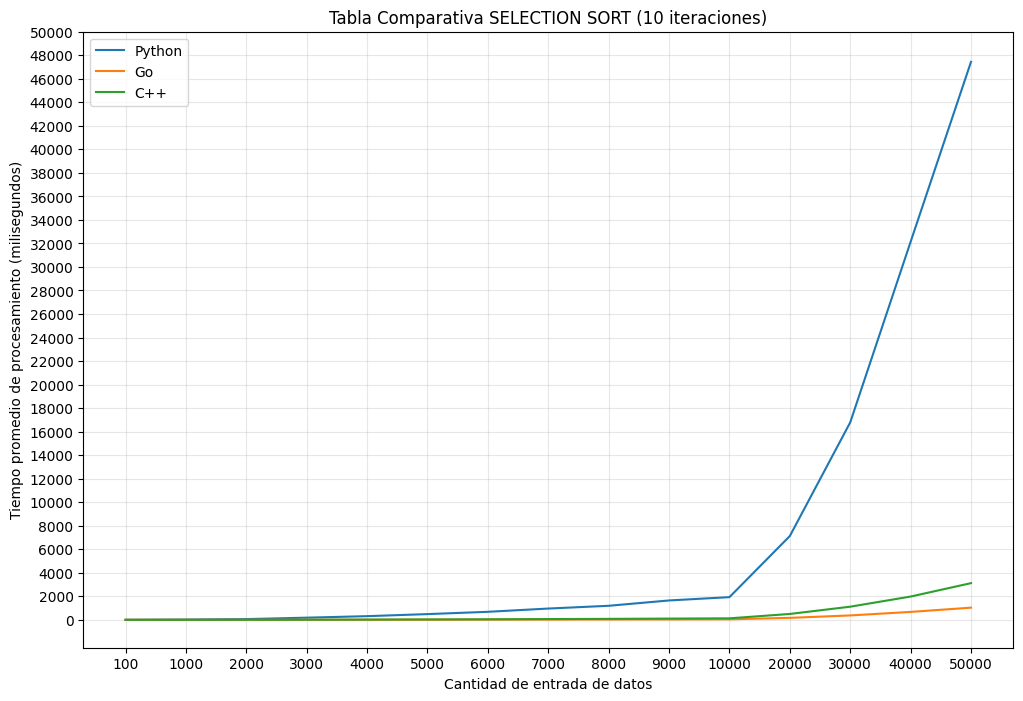
\includegraphics[width=0.95\textwidth]{imagenes/GraphicSelectionSort.png}
        \caption{\label{fig:bigOSelectionSort}Gráfica comparativa Big-O del tiempo promedio de Ejecución Selection Sort}
        \end{figure}
    \end{itemize}


% *****************************************************************

\section{CONCLUSIONES}
\begin{enumerate}
  \item Se introdujo el concepto de algoritmos y se explicaron cuatro algoritmos de ordenación: Quick Sort, Merge Sort, Bubble Sort y Selection Sort. Cada algoritmo se describió brevemente, y se detallaron sus complejidades en el mejor caso, peor caso y caso promedio.
  \item Se presentó la Notación Big-O como una forma de medir el tiempo de ejecución y la eficiencia de un algoritmo.
  \item Se introdujo la librería Matplotlib en Python, que permite crear visualizaciones animadas, estáticas e interactivas.
  \item Se realizó una comparación de costos computacionales entre los algoritmos de ordenación mencionados (Quick Sort, Merge Sort, Bubble Sort y Selection Sort) utilizando tres lenguajes de programación: Python, Golang (Go) y C++. Se presentaron tablas con los tiempos promedio de ejecución y las desviaciones estándar para diferentes tamaños de entrada de datos. Se utilizó una imagen para mostrar una comparación gráfica de sus diferentes tiempos de ejecución.
  \item Las tablas comparativas muestran que Quick Sort y Merge Sort son considerablemente más eficientes en términos de tiempo de ejecución en comparación con Bubble Sort y Selection Sort, especialmente para tamaños grandes de datos. Además, las desviaciones estándar más pequeñas indican una mayor consistencia en los resultados.
  \item Golang (Go) y C++ generalmente muestran tiempos de ejecución más bajos en comparación con Python en la mayoría de los casos, lo que sugiere que son lenguajes más adecuados para implementaciones de algoritmos que requieren un alto rendimiento.
  \item En general, se concluye que Quick Sort y Merge Sort son algoritmos más eficientes y consistentes para la ordenación de datos en comparación con Bubble Sort y Selection Sort. Además, para aplicaciones que requieren un rendimiento óptimo, Golang (Go) y C++ pueden ser opciones preferidas sobre Python.
\end{enumerate}
Es importante tener en cuenta que los resultados de tiempo de ejecución pueden variar según el hardware y el entorno de ejecución utilizado para las pruebas. Se recomienda realizar pruebas adicionales y comparaciones en un contexto específico antes de tomar decisiones finales sobre qué algoritmo y lenguaje de programación utilizar en un proyecto real.


\begin{thebibliography}{widest entry} 
  \bibitem[1]{} Mamber, U. Introduction to Algorithms. A Creative Approach
  \bibitem[2]{} Cormen, Thomas; Leiserson, Charles; Rivest, Ronald; Stein, Clifford (2009). Introduction to Algorithms (Third ed.)
  \bibitem[3]{} Cormen, Thomas; Leiserson, Charles; Rivest, Ronald; Stein, Clifford (2009). Introduction to Algorithms (Third ed.)
  \bibitem[4]{} Astrachan, Owen (2003).
  \bibitem[5]{} Knuth, Donald (1998). "Section 5.2.4: Sorting by Merging". Sorting and Searching. The Art of Computer Programming
  \bibitem[6]{} ITIS IS04: Capítulo 10. Introducción al Análisis de Algoritmos
 \end{thebibliography}

\end{document}